\documentclass[11pt,a4paper,normalheadings,twoside,DIV9,BCOR10mm,listsleft,fleqn,leqno,tablecaptionbelow,abstracton,pointlessnumbers]{scrbook}

%%\documentclass[10pt,ngerman,a4paper,normalheadings,twoside,DIV9,BCOR10mm,listsleft,fleqn,leqno,tablecaptionbelow,abstracton,pointlessnumbers]{scrbook} baris


\usepackage[T1]{fontenc}
\usepackage[latin1]{inputenc}

%package added by baris
\usepackage{verbatim} %baris to support multi line comment e.g. \begin{comment} ... \end{comment}
\usepackage[round]{natbib} %baris for bibtex http://www.economics.utoronto.ca/osborne/latex/BIBTEX.HTM
\usepackage[titletoc,toc,title]{appendix}


%% Einfache Definitionen von Konstanten f�r das gesamte Dokument.
%%  Sie werden bspw. beim Aufbau der Titelseite ausgewertet.
\def\titelname    {Personalized Mass Email Communication}
\def\autorforinfo {Baris Oztop}
%%\def\email        {oztop@in.tum.de}
\def\subjectname  {Personalized Mass Email Communication}	%Beispiel
\def\location     {M�nchen}
\def\keywordsname {email; mail merge; crowdsourcing; web application; assistant support; survey}			%Beispiel

%% spezifisch fuer eine MA, fuer BA etc. muss das angepasst werden
\def\doctype{Master's Thesis in Informatik}
\def\title{Personalized Mass Email Communication}
\def\titleGer{Personalisierte Email Massenkommunikation}
\def\author{Baris Oztop}
\def\date{August 15, 2013}

%% Festlegen der Dokumentmetrik
\usepackage[inner=2.5cm,outer=3.5cm,top=1cm,bottom=1cm,includeheadfoot]{geometry}
\usepackage{palatino}
\usepackage{amsmath}
\usepackage{amssymb}
\usepackage{amsthm}
\usepackage{amsbsy}
%%\usepackage{babel} %baris: gave error since I disabled german support at documentclass i.e. ngerman
\usepackage{paralist}
\linespread{1.6} %baris

\usepackage{xspace}
\tolerance=500   % Verhindet pingelige "`overfull \hbox"'-Meldungen.

%% Bereich Tabellen
\usepackage{array}
\usepackage{booktabs}
\usepackage{colortbl}
\usepackage{everysel}
\usepackage{framed}
\usepackage{ragged2e}
\usepackage{multirow} %baris
\usepackage{bigstrut} %baris
\usepackage{tabulary} %baris
\usepackage{longtable} %baris
%%\usepackage[table]{xcolor} %baris
%%\definecolor{lightgray}{gray}{0.9}
%%\usepackage{floatrow} %baris following two lines belong to this line
%%\DeclareFloatFont{tiny}{\tiny}% "scriptsize" is defined by floatrow, "tiny" not
%%\floatsetup[table]{font=tiny}

%% Einbindung von Minitocs
%\usepackage{shorttoc}
\usepackage{minitoc}

%% Flexible Tabellenspalten und Kommandos
\newcolumntype{L}{>{\RaggedRight\arraybackslash}X}%
\newcolumntype{C}{>{\Centering\arraybackslash}X}%
\newcolumntype{R}{>{\RaggedLeft\arraybackslash}X}%

\newcommand{\opentableheader}{\toprule}
\newcommand{\closetableheader}{\toprule}

%% actual versions of the listings package:
%% ftp://ftp.dante.de/tex-archive/help/Catalogue/entries/listings.html
\usepackage{listings}
%%\usepackage{dotnet_new}
\usepackage[pdftex, colorlinks,
            linkcolor=black,
            citecolor=black,
            pagecolor=black,
            filecolor=black,
            urlcolor=black]{hyperref}
\usepackage{graphicx}

%%\usepackage{bibgerm}
%%\usepackage{array}
%%\usepackage{colortbl}
%%\usepackage{longtable}
\usepackage[final]{pdfpages}

%% Benutzen der Koma-Headings
\usepackage[komastyle]{scrpage2}

%% kompakte Items
\usepackage{paralist}

%% verbatin in footnode
\usepackage{fancyvrb} 

%% Eigene Packages
%%%
%%% Abk�rzungen
%%%

%%% Referenzierungshilfen


%%% Fachbegriffe
\newcommand{\vmxt}{V-Modell~XT}
\newcommand{\vmx}{V-Modell}




\newcommand{\JEE}{Java~2 Plattform Enterprise Edition}
\newcommand{\JSE}{Java~2 Plattform Standard Edition}
\newcommand{\DOTNET}{.{\@}NET}
\newcommand{\COMPLUS}{COM+}
\newcommand{\Cpp}{C++}
\newcommand{\CSHARP}{C\#}
\newcommand{\ES}{\emph{Enterprise Services}}
\newcommand{\Rem}{\emph{.NET Remoting}}

%%% (kommerzielle) Produkte
\newcommand{\productname}[1]{#1}
\newcommand{\iis}{\productname{IIS}}
\newcommand{\IIS}{\productname{Internet Information Services}}
\newcommand{\VSN}{\productname{Visual Studio.NET}}
\newcommand{\BCB}{\productname{Borland C\#~Builder}}
\newcommand{\BJB}{\productname{Borland JBuilder}}

%%% Makros
\newcommand{\kw}[1]{\texttt{#1}}  % weil ich faul bin...
\newcommand{\method}[1]{Methode \texttt{#1()}}
% etwa: "\method{create}\ zeigt...", nicht: "Die \method{create}"=Methode..."

%%% f�r Bewertungen und Checklisten (zB in Tabellen)

\newcommand{\EVp}{+\xspace}   % +
\newcommand{\EVpp}{++\xspace}   % ++
\newcommand{\EVppp}{+++\xspace}   % +++
\newcommand{\EVm}{--\xspace}   % -
\newcommand{\EVmm}{{--}{--}\xspace}   % --
\newcommand{\EVmmm}{{--}{--}{--}\xspace}   % ---
\newcommand{\EVneutral}{--{\slash}+\xspace}   % -
\newcommand{\CHyes}{\ding{51}}  % yes, Haken
\newcommand{\CHno}{--}  % no


%%% Abk�rzungen - Floskeln
% Die Makros sollten eingesetzt werden, um die W�rter als Abk�rzungen zu nutzen.
% Wenn man also "`vergleiche"' ausgeschrieben haben will, dann muss
% man dieses Wort voll ausgeschreiben.
%
% Der Einsatz ist Geschmacksache, bei einigen Sachen aber sinnvoll.

\newcommand{\vgl}{vgl.\@}               % vergleiche
\newcommand{\etc}{etc.\@}               % Achtung: am Satzende nicht verwenden!
\newcommand{\evtl}{evtl.\@}             % eventuell
\newcommand{\bspw}{bspw.\@}             % beispielsweise
\newcommand{\oa}{o.\,a.\@}              % ...
\newcommand{\zB}{z.\,B.\@}
\newcommand{\zT}{z.\,T.\@}
\newcommand{\zZt}{z.\,Zt.\@}
\newcommand{\ua}{u.\,a.\@}
\newcommand{\ca}{ca.\@}
\newcommand{\dhx}{d.\,h.\@}
\newcommand{\usw}{usw.\@}
\newcommand{\bzw}{bzw.\@}
\newcommand{\bzgl}{bzgl.\@}
\newcommand{\Bzgl}{Bez�glich\@}
\newcommand{\sog}{sog.\@}
\newcommand{\ggf}{ggf.\@}
\newcommand{\Ggf}{Gegebenenfalls}
\newcommand{\vs}{vs.\@}
\newcommand{\engl}{engl.\@}             % englisch (z.B. f�r Wortbedeutungen...)
\newcommand{\inkl}{inkl.\@}
\newcommand{\teilw}{teilw.\@}
\newcommand{\idR}{i.\,d.\,R.\@}
\newcommand{\iS}{i.\,S.\@}
\newcommand{\uU}{u.\,U.\@}
\newcommand{\dW}{des Weiteren}
\newcommand{\DW}{Des Weiteren}
\newcommand{\iFx}{im Folgenden}
\newcommand{\IFx}{Im Folgenden}

%% GKa 2009-06-10: paar weitere commands speziell fuer diesen TR
\newcommand{\PET}{Process Enactment Tool Framework}
\newcommand{\WP}{Werkzeug Provider}
\newcommand{\TP}{Tool Provider}


%%%
%%% Eigene Kommandos und Umgebungen
%%%

% page clearing
\newcommand{\clearemptydoublepage}{%
  \ifthenelse{\boolean{@twoside}}{\newpage{\pagestyle{empty}\cleardoublepage}}%
  {\clearpage}}

%% Neuformatierung der Absatztrennung
%  Abs�tze haben 0pt Einzug und sind mit vert. Abstand
%  voneinander separiert
\setlength\parskip{\smallskipamount}
\setlength\parindent{0pt}

%% Redefinition Typewriter Font = kleinere Schrift und Silbentrennung
\renewcommand\texttt[1]{\small\ttfamily\hyphenchar\font=\defaulthyphenchar #1{}\normalsize\rmfamily\hyphenchar\font=\defaulthyphenchar}


%% verbatin in footnode
\VerbatimFootnotes


%%Colors
\definecolor{brightgray}{gray}{0.9}
\definecolor{darkgray}{gray}{0.5}
\definecolor{darkgreen}{rgb}{0.0,0.5,0.0}
\definecolor{dg}{rgb}{0.0,0.5,0.0}  %% dark green (Kommentare in listings)
\definecolor{dr}{rgb}{0.5,0.0,0.0}  %% dark red

% Footnote without a marker http://tex.stackexchange.com/questions/30720/footnote-without-a-marker
\newcommand\blfootnote[1]{%
  \begingroup
  \renewcommand\thefootnote{}\footnote{#1}%
  \addtocounter{footnote}{-1}%
  \endgroup
}

%\graphicspath{{imgs/}} % baris for inkscape exported odf images to find their paths
%% enable TUM symbols on title page
\usepackage{tumlogo}

%% some information for acrobat reader
\pdfinfo{%
%%  /Title (\titelname)
  /Author (\autorforinfo)
  /Subject (\subjectname)
  /Keywords (\keywordsname)
}
\clearscrplain
%% end of preamble

%% beginning of document
\begin{document}
\pagestyle{scrplain}

%%\frontmatter
% The front cover for the TUM report document.
% Included by MAIN.TEX


%--------------------------------------------------
% The Front Cover
%--------------------------------------------------

% The front cover for the TUM document.
% Included by MAIN.TEX


%--------------------------------------------------
% The Front Cover
%--------------------------------------------------

% correct BCOR - undo at the end !!!
\def\bcorcor{0.15cm}
\addtolength{\hoffset}{\bcorcor}

\thispagestyle{empty}

 \vspace{4cm}
\begin{center}
	       \oTUM{4cm}
	   
	   \vspace{5mm}     
	   \huge FAKULT{\"A}T F{\"U}R INFORMATIK\\ 
	   \vspace{0.5cm}
	 \large DER TECHNISCHEN UNIVERSIT{\"A}T M{\"U}NCHEN\\
    \vspace{1mm}
        
	\end{center}
		

\vspace{15mm}
\begin{center}

   {\Large \doctype}

  \vspace{20mm}
  
  {\LARGE  \bf \titleGer}\\%[3ex]
  
  
  \vspace{15mm}
  
  
  {\LARGE  \author}
  
  \vspace{10mm}
  
  \begin{figure}[h!]
  \centering
   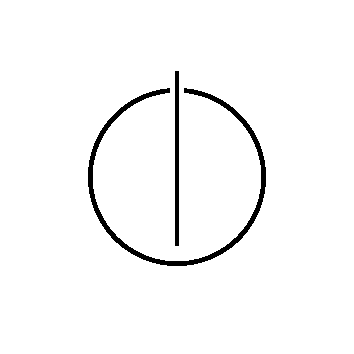
\includegraphics[width=4cm]{imgs/informat.png}
  \end{figure}
  
  \end{center}

\clearemptydoublepage
% The titlepage for the CAMP report document.
% Included by MAIN.TEX


%--------------------------------------------------
% The title page
%--------------------------------------------------

% correct BCOR - undo at the end !!!
\def\bcorcor{0.15cm}
\addtolength{\hoffset}{\bcorcor}

\thispagestyle{empty}

 \vspace{10mm}
\begin{center}
	       \oTUM{4cm}
	   
	   \vspace{5mm}     
	   \huge FAKULT{\"A}T F{\"U}R INFORMATIK\\ 
	   \vspace{0.5cm}
	 \large DER TECHNISCHEN UNIVERSIT{\"A}T M{\"U}NCHEN\\
        
	\end{center}
		

\vspace{10mm}
\begin{center}

   {\Large \doctype}

  \vspace{12mm}
  
  {\Large \bf \titleGer}\\
  
  
  \vspace{12mm}
  
  
  {\Large \bf \title}\\
  
  
  \vspace{20mm}

    %\hfill
    \begin{tabular}{ll}
	   \large Author:     & \large \author \\[2mm]
	   \large Supervisor:    & \large Prof. Dr. Johann Schlichter \\[2mm]				
	   \large Advisor:	& \large Dr. Wolfgang W{\"o}rndl \\[2mm]
	   \large Submission:       & \large August 15, 2013
	 \end{tabular}
	 
	 \vspace{5mm}
	 
	 \begin{figure}[h!]
  \centering
   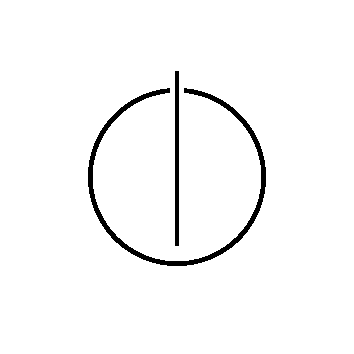
\includegraphics[width=4cm]{imgs/informat.png}
  \end{figure}
   

\end{center}

% undo BCOR correction
\addtolength{\hoffset}{\bcorcor}
\pagenumbering{roman}\setcounter{page}{1}
\documentclass[]{article}
\usepackage{natbib}
\usepackage[latin1]{inputenc}

\begin{document}

\title{Title}
\author{Author}
\date{Today}
\maketitle

\section{Introduction}

\cite{Babbie2010}
\cite{BachmannD.ElfrinkJ.&Vazzana1999}
\cite{Barron2002}
\cite{Bogen1996}
\cite{Bradburn1978}
\cite{Dillman2006}
\cite{Dillman1991}
\cite{DillmanDonA.SmythJoleneD.Christian2009}
\cite{Dillman1974a}
\cite{Emerson1976}
\cite{Groves2009}
\cite{Heberlein1978}
\cite{Heerwegh2005}
\cite{Joinson2007}
\cite{Lewis1993}
\cite{Madden2003}
\cite{Madden2008}
\cite{Mavis1998}
\cite{InternetWorldStats2012}
\cite{Norman2000}
\cite{Paolo2009}
\cite{Purcell2011}
\cite{Schaefer1998}
\cite{Scott1969}
\cite{Sheehan2006}
\cite{Sproull1986}
\cite{Sue2011}
\cite{Zikmund2007}

\bibliographystyle{plainnat}
\bibliography{collection4}

\end{document}
% Acknowledgements for the TUM report document
% Included by MAIN.TEX

\clearemptydoublepage
\phantomsection
\addcontentsline{toc}{chapter}{Acknowledgements}	

%\vspace*{2cm}
%{\Large \bf Acknowledgements}
%\vspace{1cm}
\chapter*{Acknowledgements}

Acknowledgements goes here

% Abstract for the TUM report document
% Included by MAIN.TEX

%\clearemptydoublepage
\phantomsection
\addcontentsline{toc}{chapter}{Abstract}	

%\vspace*{2cm}
%{\Large \bf Abstract}
%\vspace{1cm}
\chapter*{Abstract}

Reaching out to large-scale of people via Internet is a fast and cost efficient way compared with postal mail or telephone. Therefore, email has been used not just for research, but also for marketing, customer support, and other data collection purposes. However, getting an acceptable response rate on the sent out emails requires additional efforts from the researchers' side. This thesis investigates a communication system, which contributes to increasing the response rate while minimizing the burden on the researchers' side. 
\vspace{1cm}

To achieve this, the system constructs a workflow supporting researchers to extract information, providing rule based automated decision making mechanism on respondents' emails, and personalize the content of the emails with the respondents' information which is extracted from the current state or earlier conversations. It also provides an option to enable contribution of other researchers as assistants to interact with the workflow under the permission of the initial researcher. Therefore, distribution of the work can ease individual's efforts on the mass email communication. This feature can be further extended by enabling crowd assistants to contribute to nearly all phases of the communication flow, and getting guidance or assistance by the initial researcher when it requires.
\vspace{1cm}

This thesis demonstrates that providing a proper workflow and the possibility of an assistant contribution, a mass email communication can be achieved as if each email is individually tailored to each recipient, which contributes to high response rates. Therefore, while it minimizes the efforts on the creation of emails, it maximizes the scale on the number of people communicated to.


\clearscrplain

%% table of contents
\clearscrheadfoot
\ohead{\headmark}
\ofoot[\pagemark]{\pagemark}
\automark[chapter]{section}

%% Konfiguration der Minitocs
\dominitoc
\setcounter{minitocdepth}{3}
\mtcsettitle{minitoc}{�bersicht}
\mtcsettitlefont{minitoc}{\large\sffamily}
\mtcsetfont{minitoc}{*}{\sffamily}
\mtcsetfont{minitoc}{section}{\normalfont}
\mtcsetfont{minitoc}{subsection}{\normalfont}
\mtcsetfont{minitoc}{subsubsection}{\normalfont}

%% Erstellen der Inhaltsverzeichnisse, Tabellen und Bilder (Listings opt.)
\tableofcontents
\vfill
\cleardoublepage

\addcontentsline{toc}{chapter}{List of Figures}	
\listoffigures
\cleardoublepage

\addcontentsline{toc}{chapter}{List of Tables}
\listoftables
\cleardoublepage

\lstlistoflistings
\cleardoublepage

\clearscrheadfoot
\ohead{\headmark}
\ofoot[\pagemark]{\pagemark}
\automark[chapter]{section}
\renewcommand{\headfont}{\normalfont\sffamily\slshape}
\renewcommand{\pnumfont}{\normalfont\sffamily}

%\renewcommand{\baselinestretch}{1.25}\normalsize

\pagestyle{scrheadings}
\pagenumbering{arabic}\setcounter{page}{1}

%% Text: Content

\clearemptydoublepage
\phantomsection

\chapter{Introduction}
\label{chp:Intro}
Increased Internet usage turned email into a tool for communication, replacing telephone calls and regular mail \citep{Norman2000,Madden2003}. Email is used in many ways, proving that it plays a huge role in the communication world. Email is popularly used in; marketing, for engaging with clients; customer support, for offering aftersales assistance; research, on gathering the opinion of people on a certain topic; and many other cases showing that email has essentially become a part of our daily lives.
\vspace{1cm}

However, as the number of people you want to reach increases, the way on how you compose emails and extract information changes. Because, each email response should be uniquely composed based on the flow of the conversation to effectively deliver which require an increased personal effort and time on the part of the researchers. As a result, researchers tend to use online tools or third-party applications on sending out generic emails to their recipients with non-adequate personalization, which is known as one important factor needed to increase response rates \citep{Dillman1991,Schaefer1998}. Such emails are treated with a low priority, which results to low response rates at the end \citep[page 272]{DillmanDonA.SmythJoleneD.Christian2009}.
\vspace{1cm}

There are several products in the market focusing on email communication and data collection. A \ac{CRM} application keeps track of a company's communication with their clients. A help desk application offers a platform on helping solve customers' problems and provide guidance regarding products. Email marketing applications help on sending out commercial messages to groups of people. Finally, survey applications aid on conducting online surveys in getting people's views and opinions. The similarity of all these applications is that they all focus on email communications. However, none of these mentioned tools are capable of offering a complete workflow in helping out a researcher communicate with a great amount of people on a personalized level, as easy as possible by email.
\vspace{1cm}

The goal of this study is to understand the possible workflow of a personalized mass email communication, and to show that it is possible to reach a great amount of people while keeping it personalized at the same time. A complete system named Myriad has been developed to demonstrate the practical aspects of this idea.

\section{Email as a Data Collection Method}
\label{sec:1:EmailDataCol}

There is nearly a 600\% growth rate in the world-wide Internet usage between the years 2000 to 2012 that makes Europe's 63\% and North America's 80\% over-all population Internet usage proportion \citep{InternetWorldStats2012}. Email is ranked as the most popular online activity, along with search engine usage with 92\% of online adult users \citep{Purcell2011}. Also, the connectivity and the flexibility have increased with the introduction of smartphones and tablet devices \citep{Madden2008}. In addition to these facts, email is low cost and has a quick turnover compared to regular mail or telephone communication \citep{Zikmund2007}. Therefore, email as a part of communication is considered a viable option for data collection as well \citep{Zikmund2007}.
\vspace{1cm}

There are several reasons for data collection depending on the situation. However, purposes of data collection can be classified under the following categories \citep{Sue2011} \citep[pages 92--94]{Babbie2010}:

\begin{compactenum}
	\item To explore and get information about a topic
	\item To describe the events and the situations
	\item To explain things by questioning
\end{compactenum}

To illustrate these purposes and to see how we can use email to explore, describe, and explain things, let's suppose that we have an online learning platform, offering various courses publicly:

\paragraph{Exploration}
Offering online courses is relatively a new trend; therefore we do not have much previous knowledge about the topic. To explore the popularity of the platform, we would need to ask the platform's users questions such as: Why are they attending our online courses? Have they taken any online courses before? What are their income levels? Figuring out the answers to these questions will help us improve the system or to decide on its future. For example, the aggregated answers to the income level question will help us decide whether to charge the users for their usage or to offer it for free and find some sponsors to make it more viable.

\paragraph{Description}
Our goal is to describe the characteristics of the online learning platform's users. The questions that can help us to describe this can be: Where do they come from? What age range do they belong to? Were they able to attend college? With these questions, we will end up with a user profile like: between ages 16 -- 22; have never attended college, and is coming from a less developed country. Knowing our users' portfolio according to this outcome can help us to attract organizations with necessary connections in supporting such countries' young population. Hence, they can take advantage of our platform as a tool in reaching those populations, in return they monetize our platform.

\paragraph{Explanation}
With our descriptive study, we discovered out that our platform's user's age range is between ages 16 -- 22. The reasons on how our platform's users' age range turned out to be between 16 -- 22 makes up our explanatory purpose. Questions about how often they are connected to the Internet or have they attended college or a similar high level of an education institute might help us to figure out the answer on why do young people use our platform more frequently compared to older people. Collecting such statistics may help us to develop an explanation to a topic.

\vspace{1cm}
Since all of our registered users provided their email addresses as the primary and mandatory contact medium, we can send them emails to conduct our data collection whether the reason is to explore, describe or explain the user trends on our online learning platform.

\section{Problem Statement}
\label{sec:2:Problem}

To date, email, as a popular medium for communication, is utilized for many purposes such as reaching groups of people to explore, describe, and explain things. However, as the group's size gets larger, it becomes harder on the researchers' part to maintain the consistency and effectiveness of the flow of the exchange of emails as compared to that of small groups. Therefore, the researchers tend to write generic emails ignoring or using inadequate recipient specific information with the help of a third-party application or an online tool. This results into low response rates, since recipients do realize that because they are a part of a large group of people being responded to means that you will feel less important and less valued, and the chance of getting a reply is less likely to happen. On the other hand, if researchers individually tailor those emails according to their recipients, it will require a huge additional effort at an increased cost, hence reducing the advantage of using email as the primary communication medium.
\vspace{1cm}

Even though, there are many products available in the market supporting email communication, there is just no available product allowing anyone to reach larger groups via email, requiring minimum effort while keeping the communication personalized at the same time.
\vspace{1cm}

The main goal of this study is to show that a personalized email communication with large groups is possible if a proper workflow is provided. In order to achieve this goal, the study will:

\begin{compactenum}
	\item Examine the workflow of an email communication with large groups and possible exceptional cases on this flow.
	\item Investigate the effects of an email's content's personalization on the response rates.
	\item Describe how an adequate amount of personalization in emails can be supplied.
	\item Analyze the comparison of existing products claiming to provide solutions on email communication and collection of the respondents' information.
	\item Describe the design and implementation of an application satisfying the mentioned workflow to aid the researchers, including the initial prototype.
	\item Show how assistants can support the mentioned workflow. 
	\item Analyze real life usage of the application and its users' opinions about the application, and the latest statistical information giving an insight on how and in which way the application is used by its users.
\end{compactenum}
\vspace{1cm}

This study also contributes on the following areas:

\begin{compactenum}
	\item Email as a data collection method.
	\item Conducting surveys with the use of email.
	\item Defining a workflow on a mass email communication.
	\item Possible crowd-sourced assistant usage.
	\item Personalization of email content.
\end{compactenum}

\section{Outline}
\label{sec:3:Outline}

\paragraph{Chapter 1} The first chapter introduces the concept of the personalized mass email communication, defines email as a data collection medium, as well as its purposes and continues with the problem statement and the contributions of this study.

\paragraph{Chapter 2} The second chapter gives the necessary foundation on data collection by investigating related work about the email surveys, its errors, the factors affecting the response rates on a research and the studies on the personalization of emails.

\paragraph{Chapter 3} The third chapter is about existing applications available in the market and their connection with mass email communication as well as their features useful in reducing the efforts of a researcher on initiating a mass email campaign.

\paragraph{Chapter 4} The fourth chapter builds up a mass email communication scenario and introduces the prototype built upon to reflect the initial findings on a personalized mass email communication. The prototype will be reviewed, including its requirement analysis and architecture and finally, its evaluation.

\paragraph{Chapter 5} The fifth chapter will introduce the final solution, the developed and enhanced idea of the initial findings on a personalized mass email communication. The final solution will be reviewed, including its improved requirement analysis and architecture, and finally, the benefits of the solution will be described together with the experience of users with it will be brought in, with the statistical results.

\paragraph{Chapter 6} The last chapter will summarize the findings according to the chapters, and mention about the future work for the provided solution.

\clearemptydoublepage

\begin{comment}
--> We use email also more daily communication, onlar bize soru soruyor iletisim olusuyor.

(paper E21 p 442, and E5)To date, researchers have used Web page-based surveys to study large groups of on-line users (e.g. Kehoe, Pitkow and Morton, 1997) and e-mail surveys to study smaller, more homogenous on-line user groups (e.g. Parker, 1992; Smith, 1997; Tse et al, 1995). However, it appears that a relatively untapped use for the Internet is to use e-mail is to survey broader Internet populations on both a national and international basis. WRITE the problems in here as well form that paper. Problems related from researchers perspective. Also mention briefly about the purpose and design of the those surveys.


Reaching out large-scale of people via internet is a fast and cost efficient way comparing with postal mail or telephone. Therefore, email has been used not just for research, but also for marketing, customer support, and other data collection purposes. However, getting an acceptable response rates on the sent out emails requires additional efforts from the researchers' side. This thesis investigates a communication system which contributes increasing the response rates while minimizing the burden on the researchers' side. 

As aforementioned studies showed that different forms of personalization increase the response rates in email communication. However, it has become very easy to add personalized information into email thanks to the softwares. Dillman, et al. (2009) stated that over-personalization using software tools might easily result impersonal messages.

Moreover, experienced email users can identify if a message is written by a person or computer generated by looking appearance of one's name in certain locations, and similar patterns for other information \citep[page 272]{DillmanDonA.SmythJoleneD.Christian2009}. Therefore, it becomes difficult to have a correct amount and tone of personalization. The more daily interaction with digital devices will make the true authentic personalization more rare, hence achieving it will make it more important and effective \citep[page 238]{DillmanDonA.SmythJoleneD.Christian2009}.

\end{comment}
\chapter{Foundation and Related Work}
\label{chp:FouRelWor}
This chapter presents the related work on the data collection domain. Even though, the technology is different for email surveys to collect data from well-established regular mail surveying methods, the nature of the communication is similar to self-administrated questionnaires \citep{Schaefer1998}. Therefore, the chapter will also investigate the mail surveys in a way to emphasize the points which are also related with email communication, and the earlier studies on response rate influences.

\section{Surveys and Data Collection}
\label{sec:1:SurDatCol}
A Survey is defined as a system for collecting information \citep[page 3]{Sue2011}. It helps to learn about people's opinions and behaviors \citep{DillmanDonA.SmythJoleneD.Christian2009}. The produced data during or at the completion of the survey belong to the data collection process. Therefore, data collection is a fundamental step to produce useful data to enable analyzes on researches \citep[page 149]{Groves2009}. These researches include but not limited to many disciplines like sociology, statistics, psychology, marketing, economics, and heath sciences. 

\subsection{Email Surveys}
\label{sec:2.1.1:EmaSur}

Comparing many different characteristics of surveys and interviews, the concerns regarding speed and cost make the most powerful differences \citep{Sproull1986, Schaefer1998}. Email surveys offer more rapid surveying than other methods including regular mail and telephone surveys. In addition to that, email surveys are inexpensive since it removes the postage, paper and printing, and interview costs \citep{Schaefer1998}.
\vspace{1cm}

\cite{Sproull1986} identified the characteristics of email with an organizational research, within a Fortune 500 office products and systems manufacturer, who were using email for 12 years in the organization and over 80 percent of all employees in the selected unit had email access at the time of the research. Selected candidates are separated into two groups. The data collection protocol within the organization asked each of the group's participants series of questions regarding their 3-day old email inbox. Both groups filled out the questionnaire and answer open-ended questions either electronically or in writing.
\vspace{1cm}

The result of the study indicated that the average duration of data collection time for the email version was less than a week, which is half of the duration of the written version. While the response rate of the email version was 73 percent, the conventional written version's rate was 87. The percentage of missing data in the questionnaires was .2 percent in the written version, and 1.4 in the email version. There were no differences in the nature of answers in the email version comparing with the written questionnaire.
\vspace{1cm}

In another study from \cite{Sheehan2006}, where they administered only an email survey to query individuals about their online behaviors and their attitudes and opinions regarding privacy. They have reached the shortest response time with 3.65 days comparing with earlier studies conducted until that time (See table~\ref{tab:sur_res_met}).

\begin{center}
	%\renewcommand{\arraystretch}{2}
	\tiny
	\setlength{\tabcolsep}{5pt}
    \begin{longtable}{ | p{2cm} | p{2cm} | p{2cm} | p{0.75cm} | p{0.75cm} | p{1cm} | p{1cm} | p{0.5cm} | }
	\caption[Summary of Survey Research Methods Using E-mail]{Summary of Survey Research Methods Using E-mail \citep{Sheehan2006}} \label{tab:sur_res_met} \\
    
	\hline
	\multicolumn{1}{|p{2cm}|}{\textbf{Author}} & \multicolumn{1}{p{2cm}|}{\textbf{Response Sample}} & \multicolumn{1}{p{2cm}|}{\textbf{Survey Topic}} & \multicolumn{1}{p{0.75cm}|}{\textbf{Sample Size}} & \multicolumn{1}{p{0.75cm}|}{\textbf{Usable Sample}} & \multicolumn{1}{p{1cm}|}{\textbf{Method}} & \multicolumn{1}{p{1cm}|}{\textbf{Response Rate}} & \multicolumn{1}{p{0.5cm}|}{\textbf{Time (days)}} \\ \hline
	\endfirsthead
	
	\multicolumn{8}{c}%
	{{\bfseries \tablename\ \thetable{} -- continued from previous page}} \\
	\hline
	\multicolumn{1}{|p{2cm}|}{\textbf{Author}} & \multicolumn{1}{p{2cm}|}{\textbf{Response Sample}} & \multicolumn{1}{p{2cm}|}{\textbf{Survey Topic}} & \multicolumn{1}{p{0.75cm}|}{\textbf{Sample Size}} & \multicolumn{1}{p{0.75cm}|}{\textbf{Usable Sample}} & \multicolumn{1}{p{1cm}|}{\textbf{Method}} & \multicolumn{1}{p{1cm}|}{\textbf{Response Rate}} & \multicolumn{1}{p{0.5cm}|}{\textbf{Time (days)}} \\ \hline
	\endhead

	\multicolumn{8}{|r|}{{Continued on next page}} \\ \hline
	\endfoot

	\multicolumn{8}{|r|}{{*Differences not significant}} \\ \hline
	\endlastfoot

	
    \multirow{2}{2cm}{Kiesler \& Sproull (1986)}  & \multirow{2}{2cm}{Employees of a Fortune 500} & \multirow{2}{2cm}{Corporate Communication} & 115 & 77 & Mail & 67\% & 10.8 \\ \cline{4-8}
	&  &  & 115 & 86 & Email & 75\% & 9.6 \\ \hline
    \multirow{2}{2cm}{Parker (1992)}  & \multirow{2}{2cm}{Employees of AT\&T} & \multirow{2}{2cm}{Internal Communication} & 70 & 27 & Mail & 38\% & NA \\ \cline{4-8}
	&  &  & 70 & 48 & Email & 68\% & NA \\ \hline
    \multirow{2}{2cm}{Schuldt \& Totten (1994)}  & \multirow{2}{2cm}{Marketing \& MIS Professors (US)} & \multirow{2}{2cm}{Shareware Copying} & 200 & 113 & Mail & 56.5\% & NA \\ \cline{4-8}
	&  &  & 218 & 42 & Email & 19.3\% & NA \\ \hline
    \multirow{2}{2cm}{Mehta \& Sivadas (1995)}  & \multirow{2}{2cm}{Usenet Users} & \multirow{2}{2cm}{Internet Communication} & 309 & 173 & Mail & 56.5\%* & NA \\ \cline{4-8}
	&  &  & 182 & 99 & Email & 54.3\%* & NA \\ \hline
    \multirow{2}{2cm}{Tse, et al (1995)}  & \multirow{2}{2cm}{University Population (HK)} & \multirow{2}{2cm}{Business Ethics} & 200 & 54 & Mail & 27\% & 9.79 \\ \cline{4-8}
	&  &  & 200 & 12 & Email & 6\% & 8.09 \\ \hline
    \multirow{2}{2cm}{Bachman, Elfrink \& Vazzana (1996)} & \multirow{2}{2cm}{Business School Deans} & \multirow{2}{2cm}{TQM} & 224 & 147 & Mail & 65.6\% & 11.18 \\ \cline{4-8}
	&  &  & 224 & 117 & Email & 52.5\% & 4.68 \\ \hline
    Sheehan \& Hoy (1997) & University Population (Southeast US) & Privacy and New Technology & 580 & 274 & Email & 47.2\% & 4.7 \\ \hline
    \multirow{2}{2cm}{Smith (1997)} & \multirow{2}{2cm}{Web presence} & \multirow{2}{2cm}{Business Activities} & 150 & 11 & Email survey & 8\% & NA \\ \cline{4-8}
	&  &  & 150 & 42 & Email solicit & 11.3\% & NA \\ \hline
	\multirow{4}{2cm}{Schillewaert, Langerak and Duhamel (1998)} & \multirow{4}{2cm}{Web users in Belgium} & \multirow{4}{2cm}{Attitudes toward the Web} & 430 & 125 & Email & 31\% & NA \\ \cline{4-8}
	&  &  & 62.5M & 110 & Ad in magazine & 0\% & NA \\ \cline{4-8}
	&  &  & 4000 & 67 & USENET Posting & 2\% & NA \\ \cline{4-8}
	&  &  & 7500 & 51 & Hyperlinks & 0.68\% & NA \\ \hline 
    \multirow{4}{2cm}{Weible and Wallace (1998)} & \multirow{4}{2cm}{MIS Professors (US)} & \multirow{4}{2cm}{Internet Use} & 200 & 70 & Mail & 35.7\% & 12.9 \\ \cline{4-8}
	&  &  & 200 & 50 & Fax & 30.9\% & 8.8 \\ \cline{4-8}
	&  &  & 200 & 48 & Email & 29.8\% & 6.1 \\ \cline{4-8}
	&  &  & 200 & 52 & Web form & 32.7\% & 7.4 \\ \hline
    \multirow{2}{2cm}{Schaefer and Dillman (1998)} & \multirow{2}{2cm}{University Faculty} & \multirow{2}{2cm}{Unknown} & 226 & 130 & Mail & 57.5\%* & 14.39 \\ \cline{4-8}
	&  &  & 226 & 131 & Email & 58.0\%* & 9.16 \\ \hline
    \end{longtable}
\end{center}


In addition to speed of the email surveys, cost benefits have been indicated in \citeauthor{Sheehan2006}'s \citeyearpar{Sheehan2006} study also concluded that email is an extremely cost-efficient method for data collection, where the total cost estimated at \$470 (\$30 for printing out the responses, \$440 for 22 hours computer time to download surveys for printing) while postal mail is estimated at \$6,500 (printing, postage, survey, and reminder mailing).
\vspace{1cm}

In another study from \cite{Mavis1998}, the email survey was nearly seven times cost efficient than postal survey. This includes labor hours, survey materials like booklets, mailing labels, envelopes, and postage costs. Total time spent into postal survey was 33 hours, but it only required 12 hours for the email survey. Final cost was \$503.36 for postal survey, whose \$305.36 was spent for postage part, and remaining \$198 was spent for student labor cost. The only cost resulted from email survey was student labor cost, which was total \$72.
\vspace{1cm}

Moreover, \cite{Paolo2009} reported that people made longer open-ended response comments in email version of the survey compared to the mail version. While the average number of words per comment was 58.33\% in the mail version, it was 75.40\% in the email version. \cite{BachmannD.ElfrinkJ.&Vazzana1999} had the same finding in 1995 and 1998, where open-ended questions were responded more likely by email recipients than mail recipients. In the latter study conducted in 1998, researches also found that email respondents were more likely to expand their answers, even it was not suggested by the survey, resulting in more candid responses than mail surveys. Responses to open-ended questions are one of the important measure to determine the quality of the returned surveys.
\vspace{1cm}

Given these advantages and positive benefits of email surveys, the next section will provide information about survey errors.

\subsection{Survey Errors}
\label{sec:2.1.2:SurErr}
Sample surveys are quantitative estimation of the distribution of a characteristic in a population by obtaining this information from a small portion of the corresponding population \citep{Dillman1991}. To generalize results from a small portion, which is a sample, to a population, following sources of errors needs to be considered \citetext{\citealp[page 9]{Dillman2006}; \citealp{Dillman1991}}:

\paragraph{Sampling Error}
The more number of people surveyed, the larger degree of precision can be achieved. Therefore, the limitations on the number of people surveyed are considered under the sampling error. For example, while public opinion of 100 people results \(\pm\textdollar10\%\) of the true percent, 2,200 people results higher confidence with the percent of \(\pm\textdollar2\%\) \citep[page 9]{Dillman2006}. The surveys relying on predefined list of recipients considered that the list is randomly generated or with a systematic sampling. Hence, it has got little research to reduce sampling errors comparing with face-to-face interviews in which multistage cluster designs\footnote{Cluster sampling selects preexisting groups of population elements instead of a single element of the population \citep[page 106]{Groves2009}. Departments of a university or households in a block represents clusters of people. When the allocation of those sampling resources are stratified and based on multiple stages, frequently three stages, it is called multistage cluster sampling. First step selects the sample of counties, followed by the blocks within those counties, and finally the dwellings from the chosen blocks \citep{Scott1969}.} are used due to cost and time limitations \citetext{\citealp[page 106]{Groves2009}; \citealp{Dillman1991}}.

\paragraph{Coverage Error}
When the list of surveyed people does not include all the elements of the population, coverage error happens \citep[page 9]{Dillman2006}. Coverage error is considered one of the biggest issues of surveys since while surveying general public \citep{Dillman1991}.

\paragraph{Measurement Error}
When a respondent's answer is hard to evaluate or cannot be compared with other respondent's answers or there are inconsistencies between the observable variables like opinions, behaviors, or attributes and the survey responses, measurement error happens \citetext{\citealp[page 9]{Dillman2006}; \citealp{Dillman1991}}. The possible reasons might depend on poor wording or order of the questions or the characteristics of the surveyed person such as incapability to provide correct answers or motivational factors \citep{Dillman1991}.

\paragraph{Nonresponse Error}
When there are large amount of people who do not response, and their characteristics are different from the ones who responded, then it results nonresponse error \citep[page 9]{Dillman2006}. Low response has been considered a major problem, and many researches have focused on improving the response rates \citep{Dillman1991}.

\section{Response Rate Influences}
\label{sec:2.2:ResRatInf}

As mentioned in the previous section, one of the survey errors is the nonresponse error. Researchers have concerns regarding response rates, since responses coming from survey participants may be substantially different from those of nonrespondents, which will result in a biased estimate of representation of the population \citep{Bogen1996}.
\vspace{1cm}

Low response rate was even considered shortfall of the email methodology despite to its advantages \citep{BachmannD.ElfrinkJ.&Vazzana1999}. In table~\ref{tab:sur_res_met}, there are nine studies where both postal mail and email are compared side by side. Out of those nine studies, four of them show high response rate on postal mail, three of them got higher response on email and two studies did not show any significant differences. Parker's (1992) study of AT\&T employees was the only study which got an acceptably high response rate by email. \cite{Schaefer1998} attributed this fact to the novelty of email and sent emails were carefully examined instead of considered company junk email. \cite{Mavis1998} stated that studies cited by others in support of email surveys, also shown in table~\ref{tab:sur_res_met}, did not compare email data collection with more traditional methods, and their study design and analyses varied greatly. \cite{Sheehan2006} also take the attention to many of these studies' small and homogeneous population, therefore it may not represent larger population groups' response tendencies.
\vspace{1cm}

Hence, researchers investigated on how to increase response rates at email communication. \cite{Schaefer1998} conclude that even though, the technology for email is quite different from well established postal mail surveying methods, the communication is considered similar to self-administrated questionnaires delivered by post. Hence, the techniques used to increase response rates on postal mail can be applied to develop an email methodology. Following techniques are the ones where researchers focused on their effects on response rates.

\subsection{Length}
\label{sec:2.2.1:Leng}
For many people the time required to spend on survey is considered the biggest cost \citep[page 26]{DillmanDonA.SmythJoleneD.Christian2009}. The study from \cite{Heberlein1978} also states that the length of the survey has a negative effect on mail survey response rates, where they stated that each additional question reduces responses by .05\%. On the other hand, \cite{Bradburn1978} suggests that the length of the survey is correlated with its importance, therefore it will increase the efforts both on researchers and respondents side resulting a higher response rate. \cite{Bogen1996}, in his literature review, concluded that the relationship between interview length and nonresponse is weak and inconsistent.

\subsection{Multiple Contacts}
\label{sec:2.2.2:MultCont}
Researchers found that the number of attempts to contact people increases the response rates \citep{Heberlein1978,Schaefer1998}. The scenarios for multiple contacts include pre-notification contact, which is a brief notice for the main request, and follow-up contacts aiming to the people who did not respondent at the initial contact. Heberlein and Baumgertner (1978) showed that follow-up mailing has a mean return rate of 19.9\% at the initial contact, and continued with 11.9\% and 10.0\% for the second and third contacts, respectively \citep{Heberlein1978}. Schaefer and Dillman (1998) also stated the same conclusion for the multiple contacts for email in their literature research. According to this, the average response rate for email surveys with a single contact was 28.5\% while 41\% and 57\% for two and more than two contacts, respectively \citep{Schaefer1998}.

\subsection{Personalization}
\label{sec:2.2.3:Pers}
Personalization has been addressed as an important factor to increase response rates by many researchers \citep{Dillman1991,Schaefer1998}. It builds a connection between the respondent and researcher by making the respondent feel important, and drawing the respondent from out of the group \citep[page 272]{DillmanDonA.SmythJoleneD.Christian2009}. \cite{Dillman1974a} conducted a study to see the effects of personalization, where they reached half of a university alumni sample via personalized cover letters, while the other half got impersonalized letters. The personalization treatment included personal salutations and real signatures on the mails. They achieved nearly 9\% greater response rates for the personalized group. It is also stated that this type of personalization techniques can be also applied to emails \citep{Schaefer1998}. In the next section, we will continue with the applications of personalization in emails, and give the results of some studies.

\section{Personalization of Emails}
\label{sec:2.3:PersEmai}
Studies on mail surveys showed that personalization increases the response rates \citep{Dillman1991,Schaefer1998}. Personalization is also important for email communication since it builds a connection between the respondent and researcher as in the mail surveys studies, and make them feel more important and valued \citep[page 272]{DillmanDonA.SmythJoleneD.Christian2009}. With this argument, \cite{DillmanDonA.SmythJoleneD.Christian2009}, emphasized the social exchange theory\footnote{Social exchange theory was considered as a frame of reference to other theories rather than a theory by itself. It implies a two-sided, mutually contingent and rewarding transactions or exchanges \citep{Emerson1976}.} of the personalization of the email.
\vspace{1cm}

On the other hand, \cite{Barron2002} stressed on the socio psychological phenomenon, the diffusion of responsibility, which is also an outcome of volunteer's dilemma. In the volunteer's dilemma one player is needed to volunteer in order to reach the outcome preferred by all the others in the game. However, each person might be inclined to hoping that somebody else will volunteer, resulting in a higher utility of not volunteering than volunteering. According to this, the more people in the group size, the less probability of volunteering will result, which produce the diffusion of responsibility effect. In order to experiment the effect of diffusion of responsibility in the context of email requests, they sent emails asking for help either to single addresses or to a list of five addresses. In the email body (see Appendix~\ref{app:EmaiVolunDilem}), a fictitious graduate student asked a question to know if the university has a biology faculty, whose answer was well known to anyone familiar with the institute. The result of the study showed that the proportion of replies where they used single email address in the "To" field got 20\% higher response than the replies where they used groups of email addresses. In addition, the study qualified the given responses according to its helpful level, and the proportion of "very helpful" replies in the single email address condition was 187\% higher than the groups of email addresses condition.
\vspace{1cm}

Another outcome regarding using multiple email addresses in "To" field resulted concerns from respondents in the study of \cite{Selm2006}. An introductory email including a link to a web-based questionnaire was sent to recipients to explore the opinions of elderly Internet users about an electronic political debate. One of the respondents remarked his concerns regarding the confidentiality when the header of the email contained all the email addresses of the other respondents explicitly. His reaction was quoted in the study as in listing~\ref{lst:QuotReacConf}.
\vspace{1cm}

\lstset {
 %basicstyle=\footnotesize, basicstyle=\ttfamily
 frame=shadowbox,
 rulesepcolor=\color{black},
 showspaces=false,showtabs=false,tabsize=4,
 numberstyle=\tiny,
 captionpos=b,
 abovecaptionskip=1\baselineskip,
 breaklines=true,
 keepspaces=true,
 breakindent=0pt,
 columns=flexible
}

\begin{lstlisting}[float, language=, caption={[A Respondent's Reaction Regarding Confidentiality]A Respondent's Reaction Regarding Confidentiality \citep{Selm2006}}, label={lst:QuotReacConf}]
"Well, it could be good (for you) to fill in this form, but I better not. Do you want to know why? 'All responses will be treated confidentially', but what do I see in the address column? I see all the email addresses of those you've sent this message to. Do you folks call that confidentiality!? I've decided not to participate in this 'carefully composed' study, although I do have an opinion on the subject matter."
\end{lstlisting}

Even though, the authors entitled that person as "skeptical" and his reaction as a "vivid skepticism", today it is one of the biggest concerns regarding email confidentiality, and it might result in embarrassing situations from the research or the business perspective. A very recent email message (See listing~\ref{lst:EmaiMessaConfi} for the excerpt) dropped in my email inbox verifies the importance of confidentiality.  
\vspace{1cm}

\begin{lstlisting}[float, language=, caption={[An Email Message Showing the Importance of Confidentiality]An Email Message Showing the Importance of Confidentiality}, label={lst:EmaiMessaConfi}]
Dear Valued Customer,

Earlier today the email seen bellow was inadvertently sent without utilizing 'Bcc' recipients.

Our sincerest apologies for any inconvenience this may have caused you.

Kind Regards
\end{lstlisting}

In another study by \cite{Heerwegh2005}, personalization was applied to the salutations in the emails. The randomly drawn 2,540 samples from the student database of Katholieke Universiteit Leuven, Belgium were separated into equally sized two groups. In the non-personalized group, the salutation of "Dear student" was used, while in the personalized group "Dear [First name] [Last name]" was used. The email content was an invitation to a web survey which was about adolescent attitudes towards marriage and divorce. The result of the study showed that the personalization applied group got 6.9\% higher login rate to the survey than the unpersonalized group. Therefore, they concluded that increased response rates were in line with social exchange theory and with the diffusion of responsibility theory.
\vspace{1cm}

In addition to personalization of salutations on the emails, \cite{Joinson2007} stated the power of its combination with the power or status of the sender. In the study, a group of discussion panel students of Open University UK were sent an email invitation to complete a survey. Panel members were assigned to one of the conditions where salutation was modified in "Dear student", "Dear John Doe", and "Dear John". The sender power was manipulated on the first and last lines of the emails by assigning a neutral power saying that "From <name> (Strategy, Planning, and Partnerships), The Open University" and a high power "From Professor <name>, Pro-vice chancellor (Strategy, Planning, and Partnerships), The Open University". The results showed that the highest response rate was achieved when a personalized invitation came from a high power source and lowest when an impersonal one came from a neutral power source (See table~\ref{tab:pow_sal_res}). The possible reason for this was stated as personalized salutations increase people's sense of identifiability,  and its combination with a high power audience increase socially desirable, strategic behavior.

\begin{table}[!ht]
\begin{center}
	%\renewcommand{\arraystretch}{2}
	%\tiny
	%\setlength{\tabcolsep}{5pt}
	\caption[Power, salutation and response rates (raw and \%)]{Power, salutation and response rates (raw and \%) \citep{Joinson2007}} \label{tab:pow_sal_res}
    \begin{tabular}{ p{3cm} p{3cm}  p{3cm}  p{3cm} }
	\hline
	& \textbf{Dear Student} & \textbf{Dear John Doe} & \textbf{Dear John} \\ \hline
	\textbf{Neutral power} & 143 (40.1) & 158 (44.4) & 166 (46.6) \\
	\textbf{High power} & 150 (42.1) & 154 (43.3) & 190 (53.4) \\ \hline
    \end{tabular}
\end{center}
\end{table}

As aforementioned studies show different forms of personalization increase the response rates in email communication. However, it has become very easy to add personalized information into email thanks to the software. \citet[page 237-238]{DillmanDonA.SmythJoleneD.Christian2009} stated that over-personalization using software tools might easily result impersonal messages, and gave an example (See listing~\ref{lst:SampOverPersEmai}).
\vspace{1cm}

\lstset {
 %basicstyle=\footnotesize,
 frame=shadowbox,
 rulesepcolor=\color{black},
 showspaces=false,showtabs=false,tabsize=4,
 numberstyle=\tiny,
 captionpos=b,
 abovecaptionskip=1\baselineskip,
 breaklines=true,
 keepspaces=true,
 breakindent=0pt,
 columns=flexible
}

\begin{lstlisting}[float, language=, caption={[A Sample for an Over-personalized Email]A Sample for an Over-personalized Email \citep[page 237-238]{DillmanDonA.SmythJoleneD.Christian2009}}, label={lst:SampOverPersEmai}]
Dear Don Dillman,

I am writing to inform you and your wife Joye that the XYZ Company has created a new dog food that we are sure your Boston Terrier, Crickett, will find to be very tasty. 

We would like to send a free sample to your home in Pullman, Washington.

Kind regards,
XYZ
\end{lstlisting}

In this message, there is overwhelmed personalization with the usage of person's wife, their dog's type and name, and their home address. Moreover, experienced email users can identify if a message is written by a person or computer generated by looking appearance of one's name in certain locations, and similar patterns for other information \citep[page 272]{DillmanDonA.SmythJoleneD.Christian2009}. Therefore, it becomes difficult to have a correct amount and tone of personalization. The more daily interaction with digital devices will make the true authentic personalization more rare, hence achieving it will make it more important and effective \citep[page 238]{DillmanDonA.SmythJoleneD.Christian2009}.

\section{Conculusion}
\label{sec:2.4:Conc}

In conclusion, researchers conducted more mail survey studies than other survey methods to investigate data collection \citep{Dillman1991}. Some of those studies tried to answer the question of the nonresponse error, which has been considered one a major problem compared to other survey errors as discussed in section~\ref{sec:2.1.2:SurErr}. According to those mail survey studies, personalization has been addressed as an important factor to increase the response rates by many researchers in addition to other influences affecting response rates as identified in section~\ref{sec:2.2:ResRatInf}. With the advance of world-wide internet usage, researchers has been started to consider email as a data collection method, because of its cost and speed benefits compared to other data collection methods as discussed in section~\ref{sec:2.1.1:EmaSur}. However, some studies showed that response rates on email surveys are lower than on regular mail surveys despite to its advantages; in addition, it may pose a burden to researchers during the collation of responses since email communication does not emphasize on any structure like in web forms or even respondents may come up with additional clarifying questions \citep{Selm2006}. Therefore, even the technology for email is different from mail surveying methods, researchers considered the response rate influences of mail surveys for email since the communication itself is the same. In section~\ref{sec:2.3:PersEmai}, several studies applying different types of personalization are mentioned. Some of those studies modified the header of the emails to study the diffusion of responsibility. Other studies changed the salutations and signatures of the emails, which resulted in increased on response rates to the emails. On the other hand, those studies did not consider the increased awareness of recipients to the possibility of computerized personalization techniques, which results in over-personalized emails. As well as, none of the studies has taken the attention to the personal efforts of a researcher while extracting information from respondents' answers. This thesis will try to focus on those shortcomings of those studies as well, and provide a web application to overcome those issues.
\vspace{1cm}

In the next section, existing applications in the market, which leverages the email communication, will be evaluated. While some of those are focusing only email communication, as in email marketing applications, other applications like \ac{CRM} and help desk applications helped this thesis to identify the useful features that can be helpful in the area of personalized email communication.  


\begin{comment}

--> At the end of the chapter 2, a brief summary/conclusion could be helpful. Thereby, you could also put the related work in perspective to your problem statement, i.e. explaining where the existing work falls short or can be improved (by your solution).


 .... talk about dillman and finish, it is opposite idea, so keep it in this section, sonra overview of tools, de ama once be review et hocaya yolla

--> Respondendts start asking questions to clarify things E21 p446
--> bunu sorunlar kisminda yazabilirisin, niye CRM ihtiyac duydugunu acikliyor: personalization lost its effect on recent years cause of programs p152 dillman ebook 2007 - dillman kitap p237
--> E14 p379 da mail be email aslinda ayni diyor. E18 p1371 altini maviyle cizdin
--> M1, there is a table showing response rate comparison of email vs paper for many studies. USE IT
--> Mention about which of the errors are not applicable to us. Eg.g sampling since we can predefined list of people
--> 10.1.1.189.3715.pdf "Assistance: The Work Practices of Human Administrative Assistants and their Implications for IT and Organizations"speak about the assistance support
--> Bi section adi bu olsun, survey uzerine yazdiklarin bittikten sonra: The issues with email communication
--> Burden on the Researcher E21p442, bunu sonra anlat IYI

--> Talked about the 4 issues of survey in here, and those issues are applicable to emails
--> Compare Web surveys and EMail
--> write about low response rate comparing with mail
--> 7 pages, then comparison of existing products, then crowsourcing (MAYBE you can write about assistant support using Michael's paper), then first prototype, then final, mention about the improvements
--> A chapter about assistance support 10.1.1.189.3715.pdf "Assistance: The Work Practices of Human Administrative Assistants and their Implications for IT and Organizations"
--> Write about people's email life PIP_Work_Email_Report.pdf.pdf


Previously known data collection methods like regular which includes questionnaires where respondents fill and post back, or phone interviews, or face-to-face interviews have got additional options by the development of technology like web and email.
\vspace{1cm}

A first comprehensive high response rate achieved mail survey is done at 1978 \citep[page 3]{Dillman2006}.
The first web survey, which was conducted on 1994 by James E. Pitkow and Margaret M. Recker, had an aim to demonstrate that the web as a survey medium. During that that estimated internet users were only 15 million \citep{Lewis1993}. The survey was posted one of the newsgroup, and got 4,777 responses during its one month online period.

\end{comment}

%%% Local Variables: 
%%% mode: latex
%%% TeX-master: "thesis"
%%% End: 

%\appendix
\begin{appendices}
\chapter{Detailed Descriptions}
%\section{Detailed Validation Results}
\label{chapter:DetailedDescriptions}
Here come the details that are not supposed to be in the regular text.
\end{appendices}

%%\section{Literaturverzeichnis}
%% bibs...
%%\nocite{*}
\bibliographystyle{plainnat}
%%\bibliographystyle{alpha}
\bibliography{bibtex}
\vfill
%%\pagebreak

\end{document}
